% -*- latex -*-
\author{Adam Pilewski, \textbf{311382}}
\title{PGUI, Kamień milowy \\4/4}
\frenchspacing
\documentclass[a4paper,11pt]{article}

\usepackage[T1]{polski}
\usepackage[utf8]{inputenc}
\usepackage{pdfpages}
\usepackage{graphicx}
\usepackage{hyperref}
\hypersetup{
    colorlinks=true,
    linkcolor=blue,
    filecolor=magenta,      
    urlcolor=cyan,
    pdftitle={Overleaf Example},
    pdfpagemode=FullScreen,
    }

\setlength{\parindent}{0pt}
\setlength{\parskip}{\medskipamount}
\raggedbottom


\addtolength{\oddsidemargin}{-.999in}
\addtolength{\evensidemargin}{-.999in}
\addtolength{\textwidth}{2.2in}

\addtolength{\topmargin}{-.999in}
\addtolength{\textheight}{2.2in}

\begin{document}
\maketitle
\section{CodeSandbox}
\href{https://codesandbox.io/p/github/adas77/panel/main}{link do Projektu na żywo}


\section{Analiza i wymagania}
\subsection{(79h) MoSCoW}


\begin{enumerate}
    \item (47h) MUST
    \begin{enumerate}
        \item 1h Logowanie
        \item 3h Wielokontowość, generacja losowych danych
        \item 30h Stworzenie podstawowych komponentów i dostosowanie ich do używania w innych (atomic design) 
        \begin{enumerate}
            \item 10h Atomy, molekuły
            \item 3h Widget Porady
            \item 6h Widget Wykres
            \item 3h Widget Opinie
            \item 3h Widget Rankig
            \item 3h Widget Jakość
            \item 2h Widget Zamówienia
        \end{enumerate}
        \item 5h Skomponowanie stron z gotowych elementów, nawigacja
        \item 4h Interakcja z wykresem
        \item 3h Przeglądanie dostępnych danych / filtrowanie / sortowanie
    \end{enumerate}
    \item (20h) SHOULD
    \begin{enumerate}
        \item 5h Figma
        \item 6h Diagramy UML
        \item 3h Wielojęzyczność
        \item 1h Light/Dark Mode
        \item 5h Dopracowanie CSS
    \end{enumerate}
    \item (7h) COULD
    \begin{enumerate}
        \item 2h zmiana danych w czasie na Widgetach (Opinie, Wykresy)
        \item 5h dodanie animacji
    \end{enumerate}
    \item (5h) WON'T
    \begin{enumerate}
        \item 5h Wykres: Dodanie serii z zeszłego okresu i zaznaczanie punktu
        
    \end{enumerate}
\end{enumerate}

\section{UML}
% 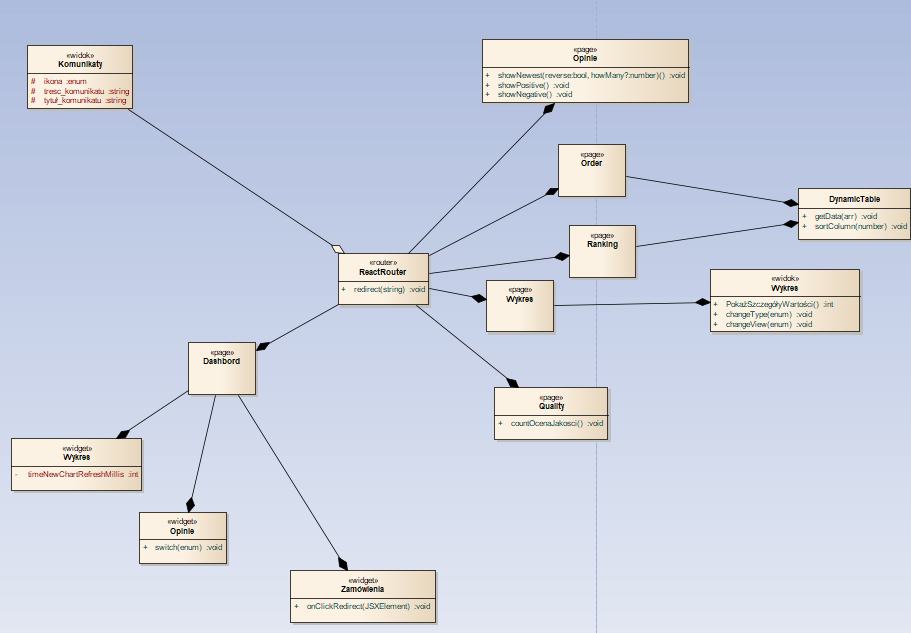
\includegraphics[scale=0.5]{src/routes.png}\\
% 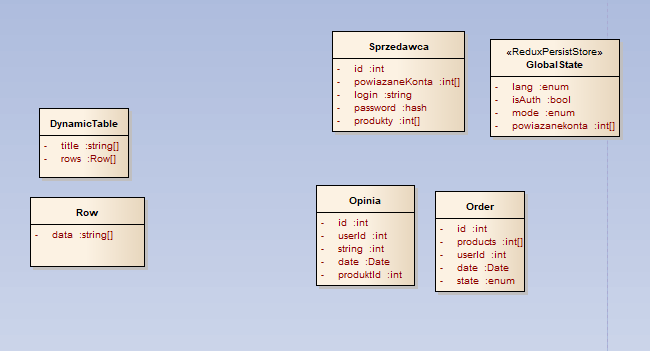
\includegraphics[scale=0.5]{src/class.png}\\
% 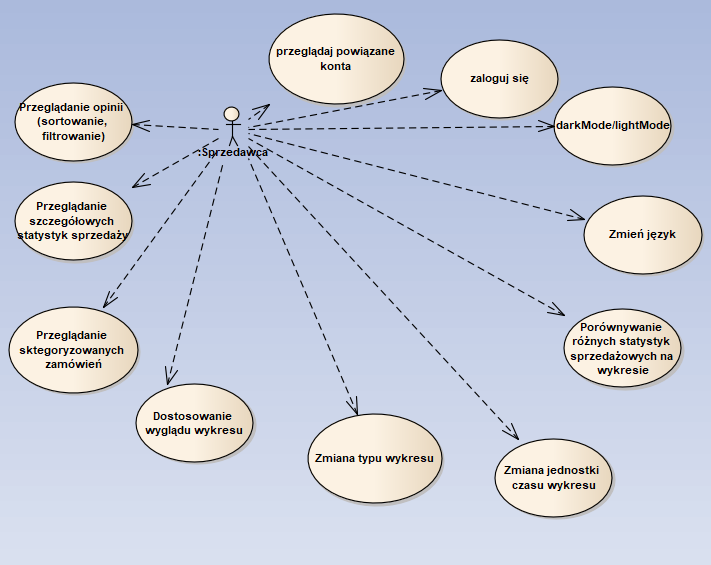
\includegraphics[scale=0.5]{src/uc.png}\\
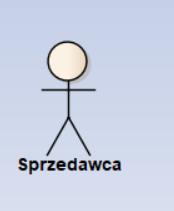
\includegraphics[scale=0.5]{src2/src2/c9.png}\\
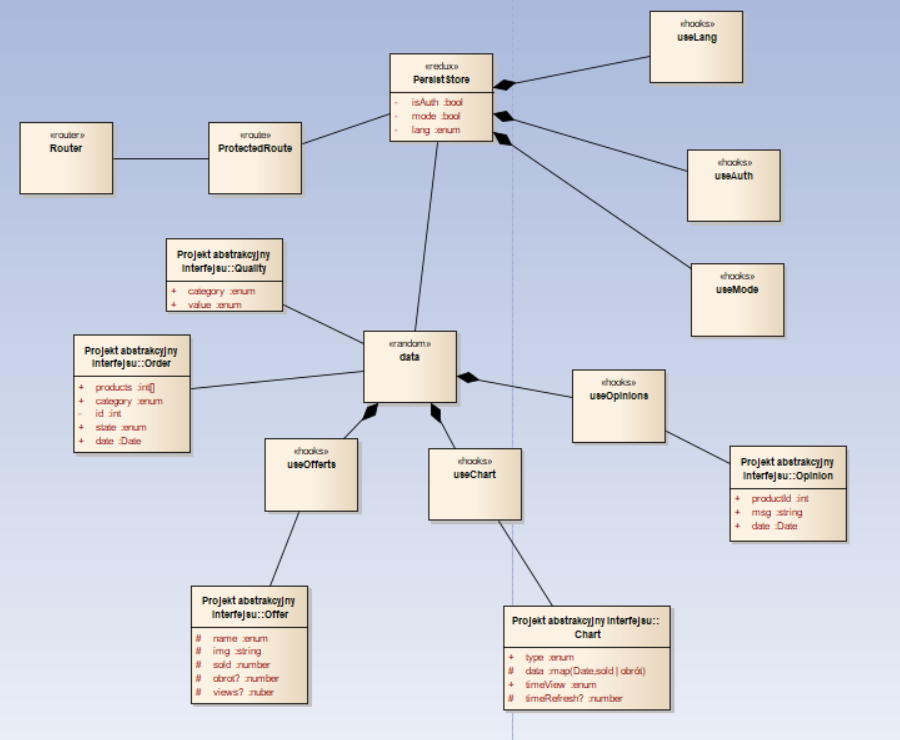
\includegraphics[scale=0.5]{src2/src2/c10.png}\\
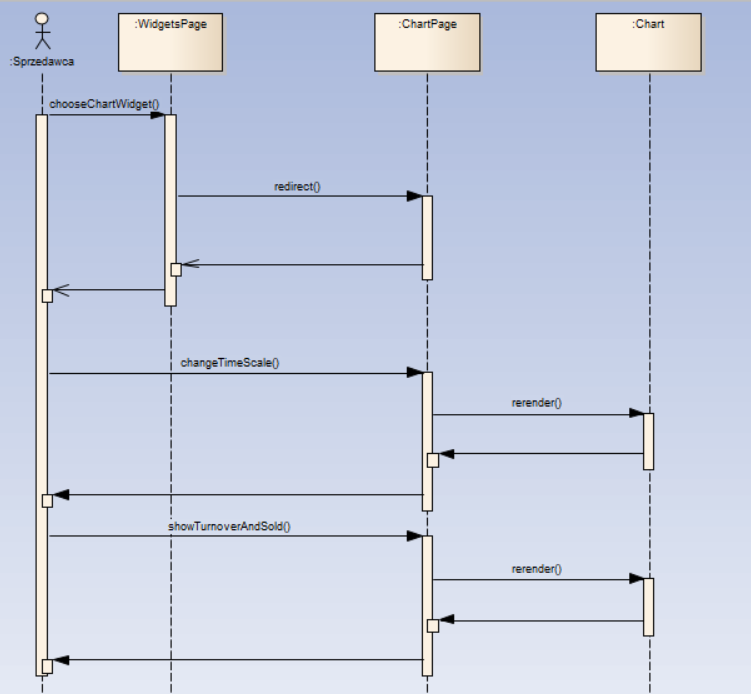
\includegraphics[scale=0.5]{src2/src2/c8.png}\\
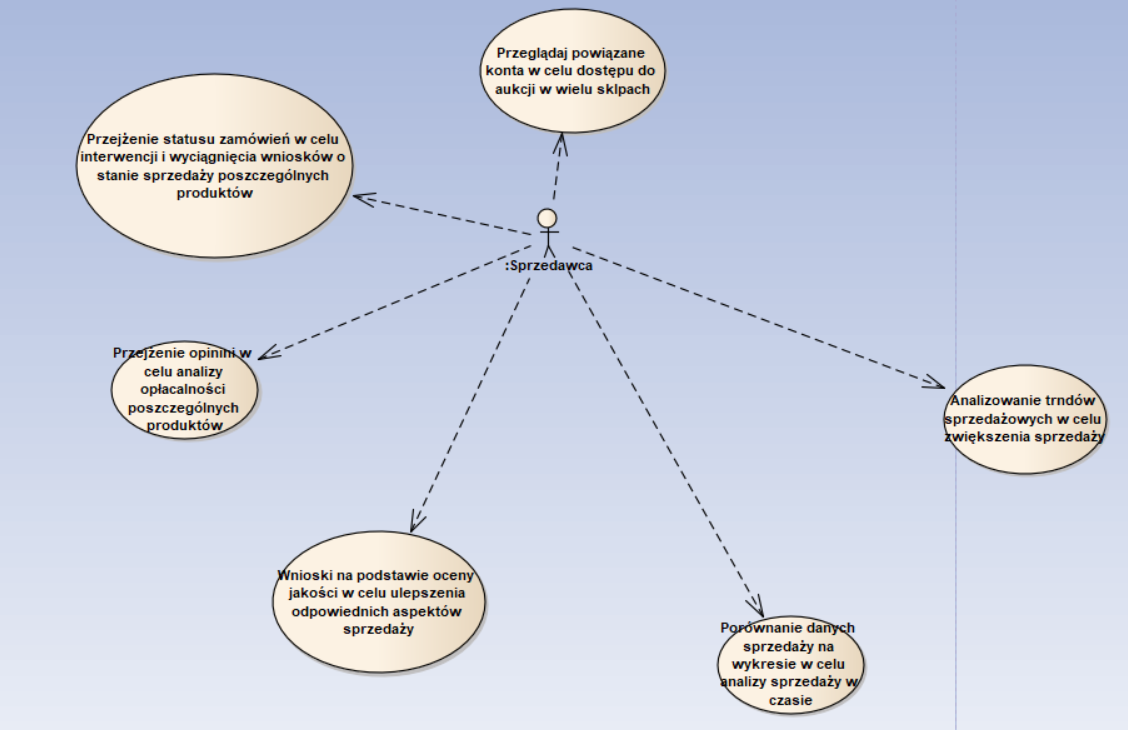
\includegraphics[scale=0.5]{src2/src2/c1.png}\\
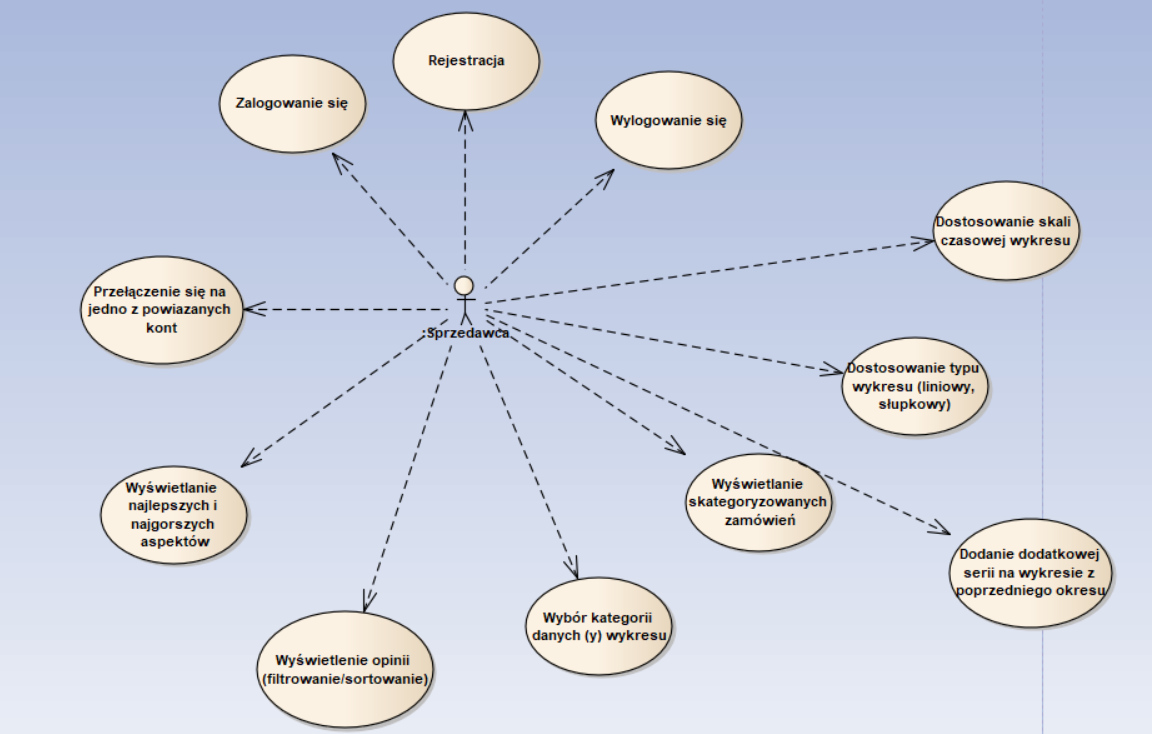
\includegraphics[scale=0.5]{src2/src2/c2.png}\\
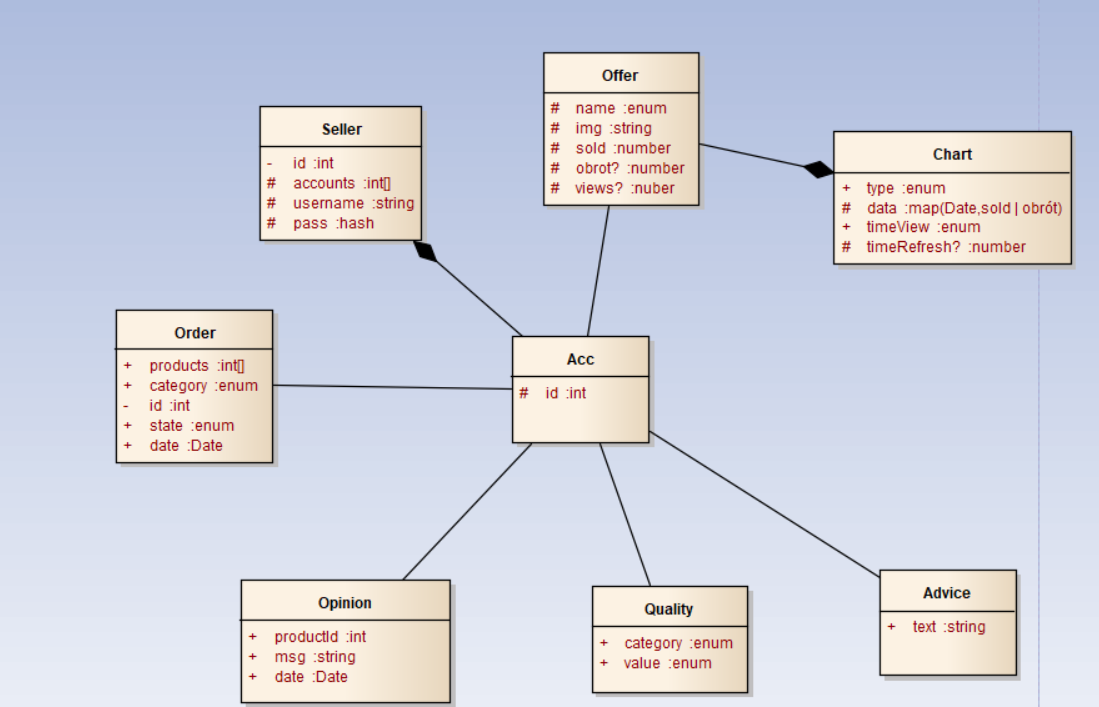
\includegraphics[scale=0.5]{src2/src2/c3.png}\\
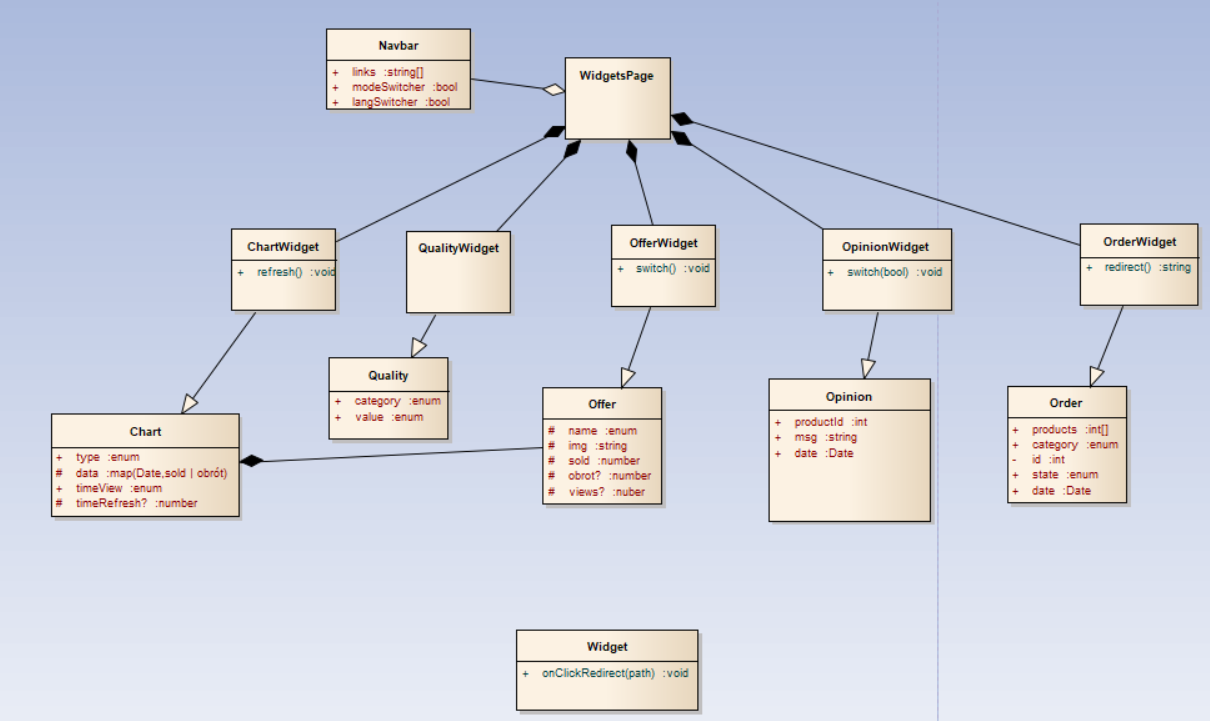
\includegraphics[scale=0.5]{src2/src2/c4.png}\\
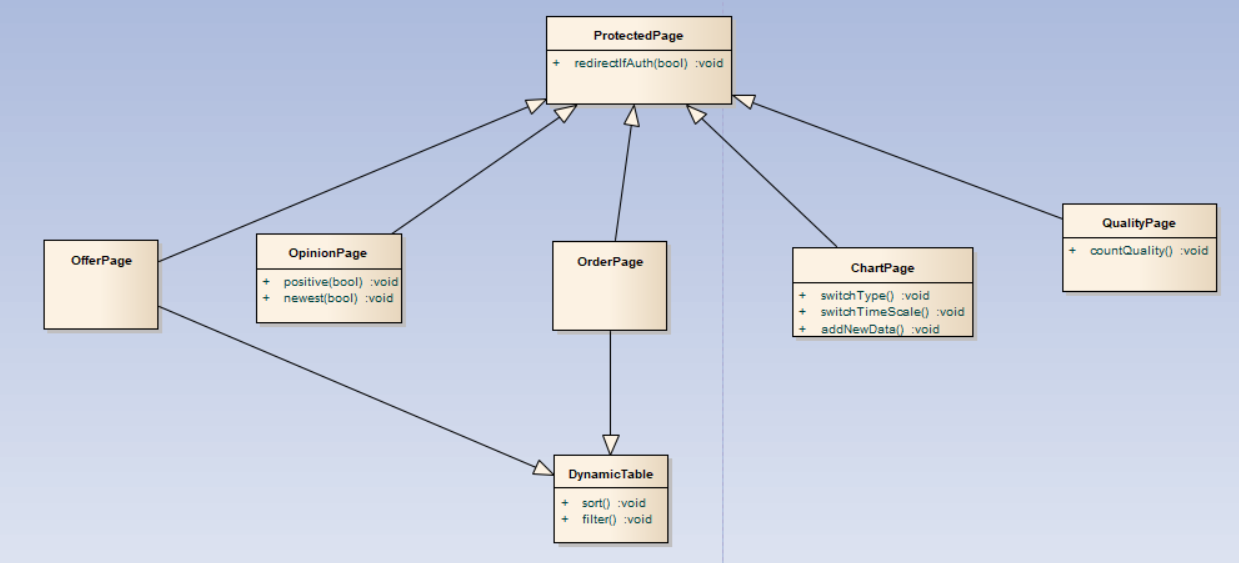
\includegraphics[scale=0.5]{src2/src2/c5.png}\\
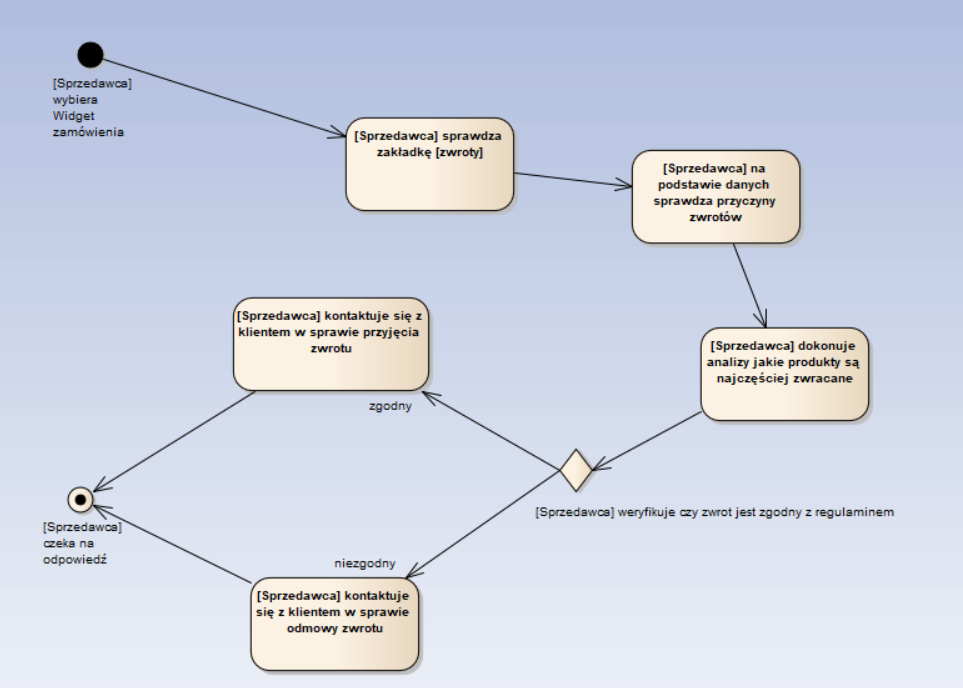
\includegraphics[scale=0.5]{src2/src2/c6.png}\\
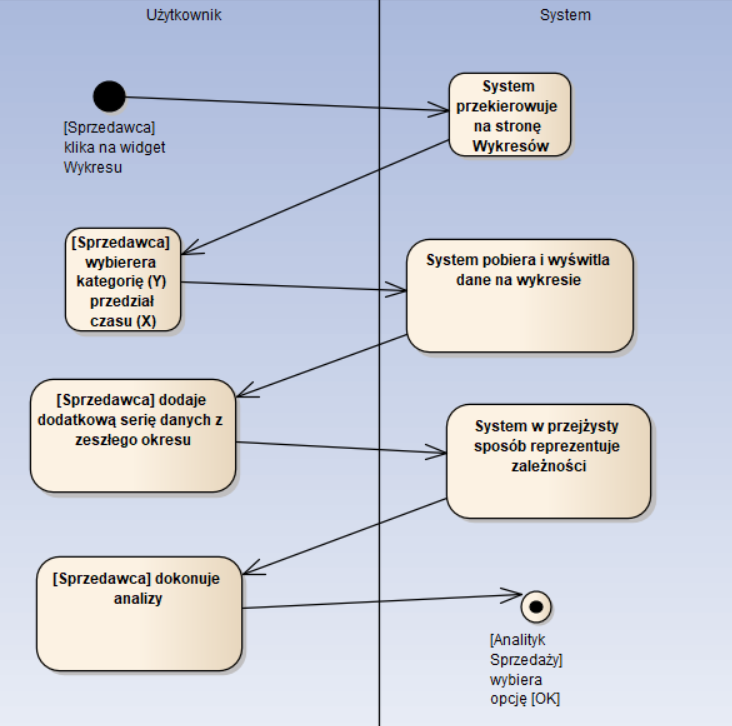
\includegraphics[scale=0.5]{src2/src2/c7.png}\\

\section{Figma}
\href{https://www.figma.com/file/6HQmM9ssZsjX2jbWcm6bmN/PGUI_PANEL_SPRZEDAWCY?node-id=0%3A1&t=sC3RxEjXZwQHD2Ov-0}{link do Figmy}
\href{https://www.figma.com/file/6HQmM9ssZsjX2jbWcm6bmN/PGUI_PANEL_SPRZEDAWCY?node-id=0%3A1&t=509EkGfDzHvN31J9-0}{link do Figmy}
\href{https://www.figma.com/proto/6HQmM9ssZsjX2jbWcm6bmN/PGUI_PANEL_SPRZEDAWCY?node-id=34%3A16652&scaling=contain&page-id=0%3A1&starting-point-node-id=34%3A16652}{link do Figmy - Prezentacja}
\section{Projekt implementacji}
\subsection{Biblioteki}
\begin{enumerate}
    \item Przechowywanie stanu
    \begin{enumerate}
        \item react-redux
        \item redux-persist
    \end{enumerate}
    \item CSS
    \begin{enumerate}
        \item tailwindcss
        \item clsx
    \end{enumerate}
    \item Nawigacja
    \begin{enumerate}
        \item react-router-dom
    \end{enumerate}
    \item Wykresy
    \begin{enumerate}
        \item recharts
    \end{enumerate}
\end{enumerate}
\subsection{Szkielet implementacji}
\url{https://github.com/adas77/panel} \\
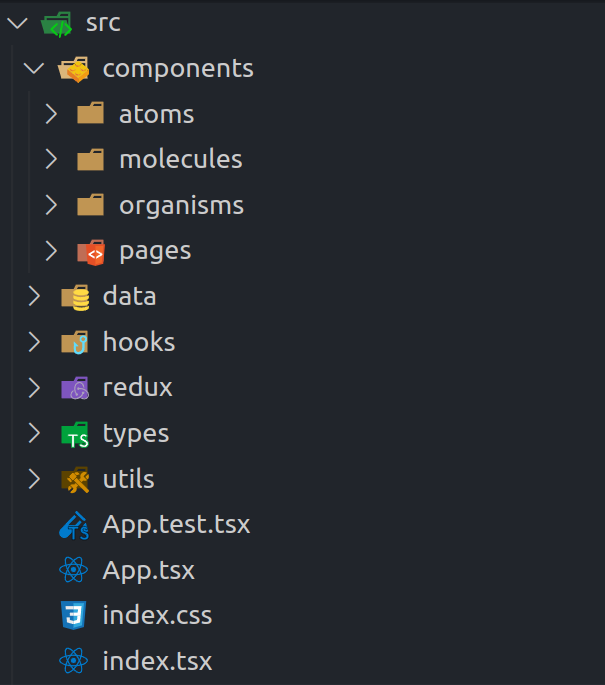
\includegraphics[scale=0.5]{src/s.png}

% \includepdf[pages=-]{src/}
% \includegraphics[scale=0.5]{src/}

\end{document}